
\documentclass[9pt]{beamer}

\mode<presentation> {

\usetheme{Madrid}

%\usecolortheme{albatross}
%\usecolortheme{beaver}
%\usecolortheme{beetle}
%\usecolortheme{crane}
%\usecolortheme{dolphin}
%\usecolortheme{dove}
%\usecolortheme{fly}
%\usecolortheme{lily}
%\usecolortheme{orchid}
%\usecolortheme{rose}
%\usecolortheme{seagull}
%\usecolortheme{seahorse}
%\usecolortheme{whale}
%\usecolortheme{wolverine}

%\setbeamertemplate{footline} % To remove the footer line in all slides uncomment this line
%\setbeamertemplate{footline}[page number] % To replace the footer line in all slides with a simple slide count uncomment this line

%\setbeamertemplate{navigation symbols}{} % To remove the navigation symbols from the bottom of all slides uncomment this line
}

\usepackage{graphicx} % Allows including images
\usepackage{booktabs} % Allows the use of \toprule, \midrule and \bottomrule in tables

%----------------------------------------------------------------------------------------
%	TITLE PAGE
%----------------------------------------------------------------------------------------

\title{ARMA-Garch Part} % The short title appears at the bottom of every slide, the full title is only on the title page

\author{Shiheng Shen, Ci Rui, Lingkun Yue} % Your name
\institute[PKU] % Your institution as it will appear on the bottom of every slide, may be shorthand to save space
{
}
\date{\today} % Date, can be changed to a custom date

\begin{document}

\begin{frame}
\titlepage % Print the title page as the first slide
\end{frame}

\begin{frame}
\frametitle{Overview} % Table of contents slide, comment this block out to remove it
\tableofcontents % Throughout your presentation, if you choose to use \section{} and \subsection{} commands, these will automatically be printed on this slide as an overview of your presentation
\end{frame}

%----------------------------------------------------------------------------------------
%	PRESENTATION SLIDES
%----------------------------------------------------------------------------------------

%------------------------------------------------
\section{Data} % Sections can be created in order to organize your presentation into discrete 


\begin{frame}
\frametitle{Data Source}
HadCRUT4 is a gridded dataset of global historical surface temperature anomalies relative to a 1961-1990 reference period. Data are available for each month since January 1850, on a 5 degree grid.
\end{frame}


\begin{frame}[fragile]
\frametitle{Read Data}
\begin{verbatim}
tmpf <- tempfile()
curl_download("http://www.metoffice.gov.uk/
hadobs/hadcrut4/data/current/time_series/
HadCRUT.4.5.0.0.monthly_ns_avg.txt", tmpf)
gtemp <- read.table(tmpf)[, 1:2]
temp = gtemp$V2[1:2004] 
plot.ts(temp)
\end{verbatim}
\end{frame}

\begin{frame}
\frametitle{Read Data}
\begin{figure}[H]
\centering
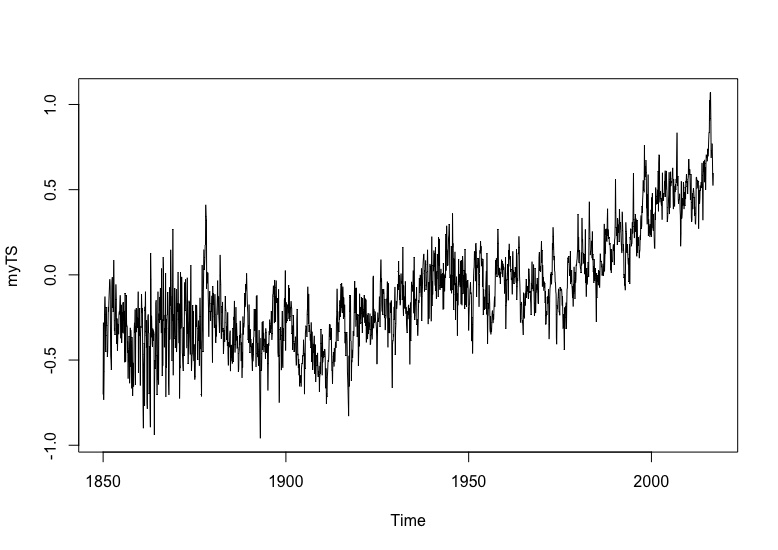
\includegraphics[scale=.45]{temp.png}
\end{figure}
\end{frame}

\section{Adjustment}

\begin{frame}[fragile]
\frametitle{Seasonal Adjusting}
\begin{verbatim}
library(TSA)
myTS = ts(as.numeric(temp), start = c(1850, 1), 
frequency = 12)
myTS.additive = decompose(myTS)
myTS.adjusted = myTS.additive$x - myTS.additive$seasonal
\end{verbatim}
\end{frame}

\begin{frame}[fragile]
\frametitle{Seasonal Adjusting}

\begin{figure}[H]
\centering
\caption{additive model: seasonal component, adjusted series}
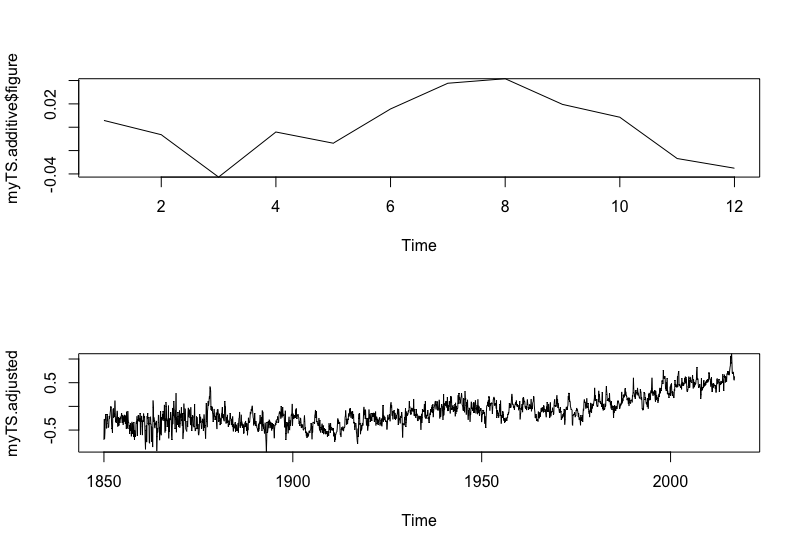
\includegraphics[scale=.30]{component.png}
\end{figure}
\end{frame}



\begin{frame}[fragile]
\frametitle{Stationarity}
\begin{verbatim}
> dtemp = diff(temp)
> adf.test(dtemp)

	Augmented Dickey-Fuller Test

data:  dtemp
Dickey-Fuller = -16.175, Lag order = 12, p-value = 0.01
alternative hypothesis: stationary
\end{verbatim}
\end{frame}

\section{ARMA Model}

\begin{frame}[fragile]
\frametitle{ARMA}
Finding the correct arma order of dtemp:
\begin{verbatim}
auto.arima(dtemp)
arma21.dtemp = arima(dtemp, c(2, 0, 1))
arma24.dtemp = arima(dtemp, c(2, 0, 4))
auto.arima(arma21.dtemp$residuals)
auto.arima(arma24.dtemp$residuals)
my.arma = arma24.dtemp
my.arma
\end{verbatim}
\end{frame}

\begin{frame}[fragile]
\frametitle{my.arma result}
\begin{verbatim}
> my.arma

Call:
arima(x = dtemp, order = c(2, 0, 4))

Coefficients:
         ar1     ar2      ma1      ma2     ma3     ma4  intercept
      0.5204  0.3247  -1.0536  -0.1269  0.1168  0.0755      5e-04
s.e.  0.2733  0.2356   0.2727   0.3828  0.1117  0.0265      2e-04

sigma^2 estimated as 0.01435:  log likelihood = 1407.67,  aic = -2801.34
\end{verbatim}
\end{frame}

\begin{frame}[fragile]
\frametitle{Test ARMA}
\begin{verbatim}
> Box.test(res, type = 'Ljung-Box')

	Box-Ljung test

data:  res
X-squared = 0.0058853, df = 1, p-value = 0.9388

> arch.test(my.arma)
ARCH heteroscedasticity test for residuals 
alternative: heteroscedastic 

Lagrange-Multiplier test: 
     order   LM p.value
[1,]     4 1418       0
[2,]     8  697       0
[3,]    12  418       0
[4,]    16  212       0
[5,]    20  168       0
[6,]    24  137       0
\end{verbatim}
\end{frame}

\begin{frame}[fragile]
\frametitle{Plot residuals}
\begin{figure}[H]
\centering
\caption{arma residual}
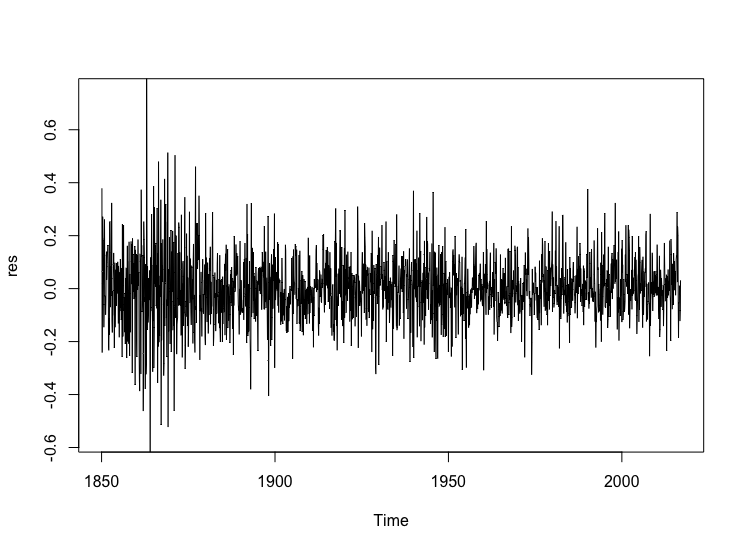
\includegraphics[scale=.40]{armares.png}
\end{figure}
\end{frame}

\section{Standard Garch Model}

\begin{frame}[fragile]
\frametitle{Building sGarch}
A standard GARCH model has the following equations:
\begin{equation*}
y_t = \mu + \sum \phi_i y_{t-i} + \sum \theta_i \epsilon_{t-j} + \epsilon_t 
\end{equation*}
\begin{equation*}
	\sigma_t^2 = (w + \sum_{j = 1}^m \zeta_j v_{jt}) + \sum_{j = 1}^q \alpha_j \varepsilon_{t-j}^2 + \sum_{j = 1}^p \beta_j \sigma_{t-j}^2
\end{equation*} 
\begin{equation*}
\epsilon_t = u_t \cdot \sigma_t, u_t \sim N(0, 1) 
\end{equation*}
\end{frame}

\begin{frame}[fragile]
\frametitle{Using \textit{rugarch} package}
\begin{verbatim}
library(rugarch)
my_sGARCH_test <- function(p, q, m, n, ts.data)
{
	# I use include.mean = FALSE after trying TRUE
	# to find out insignificance
    myspec=ugarchspec(variance.model = list(model = "sGARCH",
    	garchOrder = c(p, q)), 
    	mean.model = list(armaOrder = c(m, n), 
    	include.mean = FALSE), 
    	distribution.model = "norm")
    myfit=ugarchfit(myspec,data=ts.data, solver="solnp")
    return(myfit)  
}
\end{verbatim}
\end{frame}

\begin{frame}[fragile]
\frametitle{brief result}
\indent After trying a few times from $(1, 0), (0, 0, 0)$ to $(5, 5), (4, 0, 4)$, \textit{GARCH(1 ,1), ARIMA(2, 0, 3)} is the most satisfying model. Here we realize that using GARCH model, the order of ARIMA might changes.

\begin{verbatim}
fit1 = my_sGARCH_test(1, 1, 2, 3, dtemp)
> fit1
...
Optimal Parameters
------------------------------------
        Estimate  Std. Error    t value Pr(>|t|)
ar1    -0.090935    0.015226    -5.9724 0.000000
ar2     0.754333    0.015069    50.0583 0.000000
ma1    -0.391906    0.007313   -53.5917 0.000000
ma2    -0.863257    0.000130 -6647.5909 0.000000
ma3     0.295634    0.007800    37.9010 0.000000
omega   0.000082    0.000034     2.3956 0.016595
alpha1  0.023026    0.003614     6.3706 0.000000
beta1   0.970594    0.004705   206.2925 0.000000
...
\end{verbatim}
\end{frame}

\section{Diagnostics}

\begin{frame}[fragile]
\frametitle{diagnostics}
\indent Substract the standardized(w.r.t. the variance model) residuals $z$, which is $z = \cfrac{residuals(fit)}{sigma(fit)}$.

\begin{verbatim}
z = residuals(fit1) / sigma(fit1)
plot.ts(z)
\end{verbatim}

\begin{figure}[H]
\centering
\caption{z}
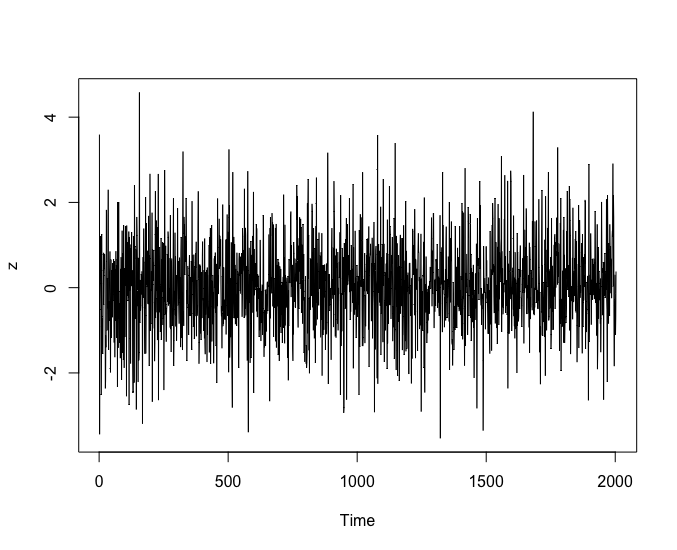
\includegraphics[scale=.20]{z.png}
\end{figure}
\end{frame}


\begin{frame}[fragile]
\frametitle{diagnostics}
\begin{verbatim}
> mean(z)
[1] 0.03181525
> var(z)
[1] 1.013866
> length(z)
[1] 2003
> plot.ts(rnorm(2003, 0.03181525, 1.013866))
\end{verbatim} 
\indent And then, just for fun, plot a normal sample series with the same parameters:

\begin{figure}[H]
\centering
\caption{simulation of using rnorm}
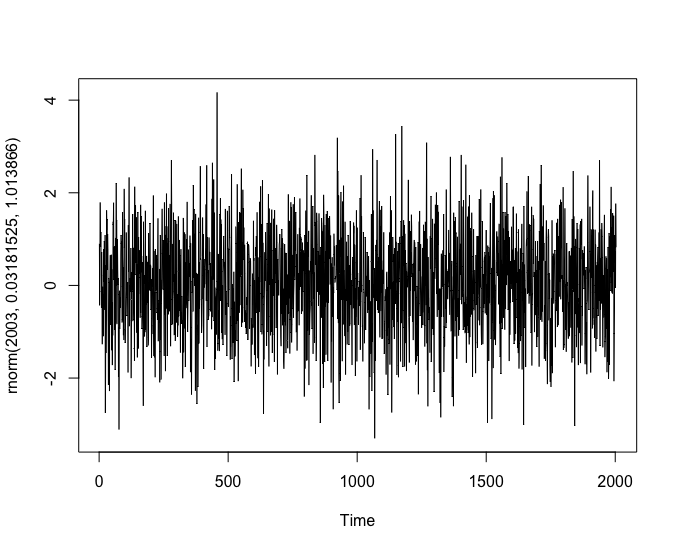
\includegraphics[scale=.20]{rnorm.png}
\end{figure}
\end{frame}



\begin{frame}[fragile]
\frametitle{diagnostics}
\begin{verbatim}
Weighted ARCH LM Tests
------------------------------------
            Statistic Shape Scale   P-Value
ARCH Lag[3]  0.004507 0.500 2.000 9.465e-01
ARCH Lag[5] 11.085543 1.440 1.667 3.565e-03
ARCH Lag[7] 20.592184 2.315 1.543 4.509e-05
\end{verbatim}
\end{frame}

\begin{frame}[fragile]
\frametitle{diagnostics}
\begin{figure}[H]
\centering
\caption{acf(dtemp)}
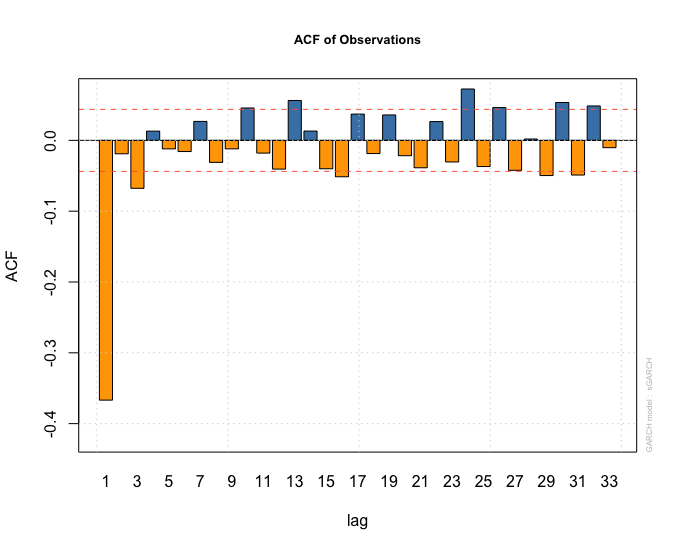
\includegraphics[scale=.30]{original_acf.png}
\end{figure}
\end{frame}

\begin{frame}
The acf of standardized residuals:
\begin{figure}[H]
\centering
\caption{acf(z)}
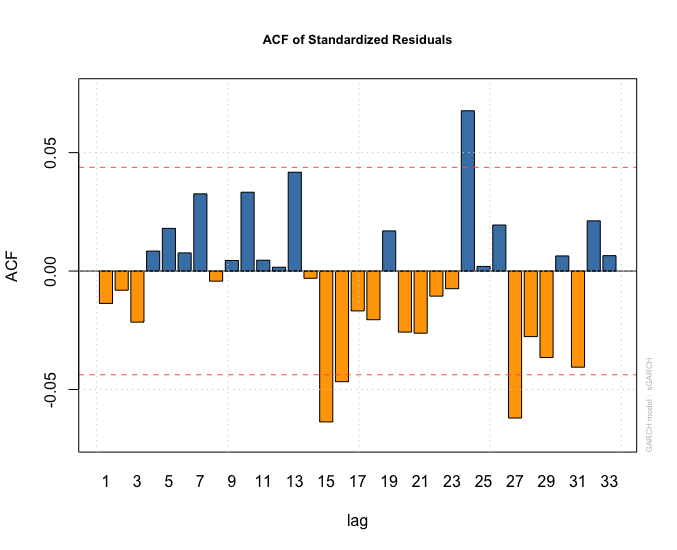
\includegraphics[scale=.30]{zacf.png}
\end{figure}
This is a prove that we should have used a long memory model.
\end{frame}

\begin{frame}[fragile]
\frametitle{diagnostics}
The \textit{Empirical Density of Standardized Residuals} compared to normal distribution:
\begin{figure}[H]
\centering
\caption{Empirical Density of Standardized Residuals}
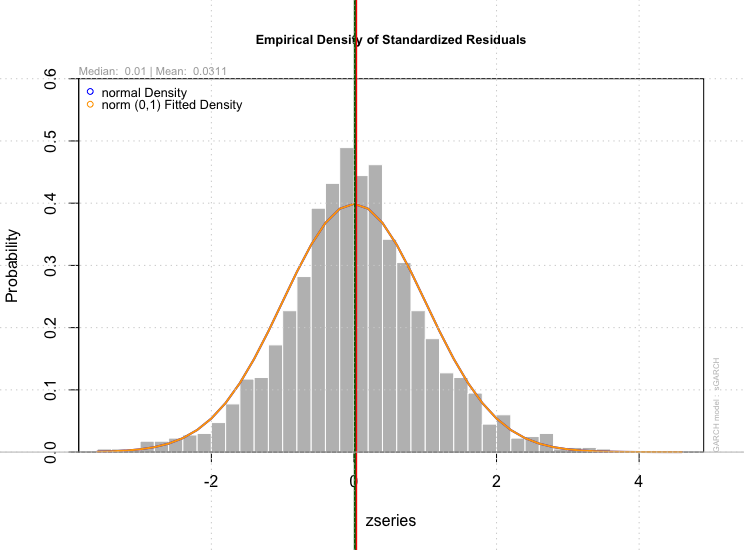
\includegraphics[scale=.35]{density.png}
\end{figure}
\end{frame}

\begin{frame}[fragile]
\frametitle{diagnostics}
qqplot:
\begin{figure}[H]
\centering
\caption{qqplot of $z$}
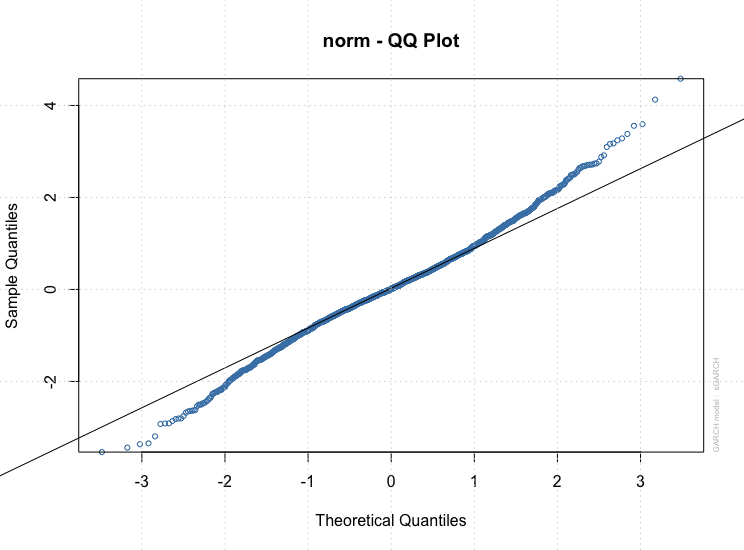
\includegraphics[scale=.35]{qqplot.png}
\end{figure}

\end{frame}

\begin{frame}[fragile]
\frametitle{diagnostics}
Series with 2 Conditional SD Superimposed:
\begin{figure}[H]
\centering
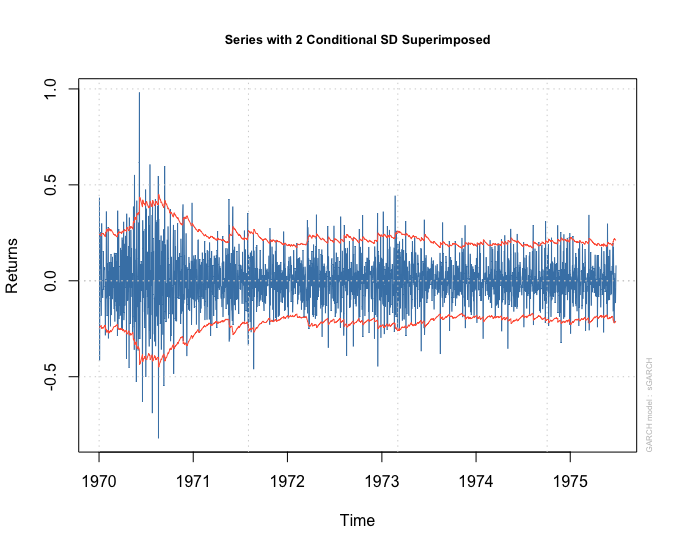
\includegraphics[scale=.40]{series_sd.png}
\end{figure}
\end{frame}

\section{Forecast}

\begin{frame}[fragile]
\frametitle{Forecast}
\begin{verbatim}
fore1 = ugarchforecast(fit1, n.ahead = 24)
fore.diff = as.numeric(fore1@forecast$seriesFor)
fore.sigma = as.numeric(fore1@forecast$sigmaFor)
ts.predict = temp[length(temp)] + cumsum(fore.diff)
ts.predict = ts.predict + myTS.additive$figure
ts.sigma = sqrt(cumsum(fore.sigma^2))
tsup.sigma = ts.predict + ts.sigma
tsdown.sigma = ts.predict - ts.sigma
plot(1:24, ts.predict, ylim=c(0,1.5), type = 'l', col = 'blue',
  xlab = "months", ylab = "temperature predict")
lines(1:24, tsup.sigma, type = 'l', col = 'red')
lines(1:24, tsdown.sigma, type = 'l', col = 'red')
\end{verbatim}
\end{frame}

\begin{frame}[fragile]
\frametitle{Forecast}
\begin{figure}[H]
\centering
\caption{forecast}
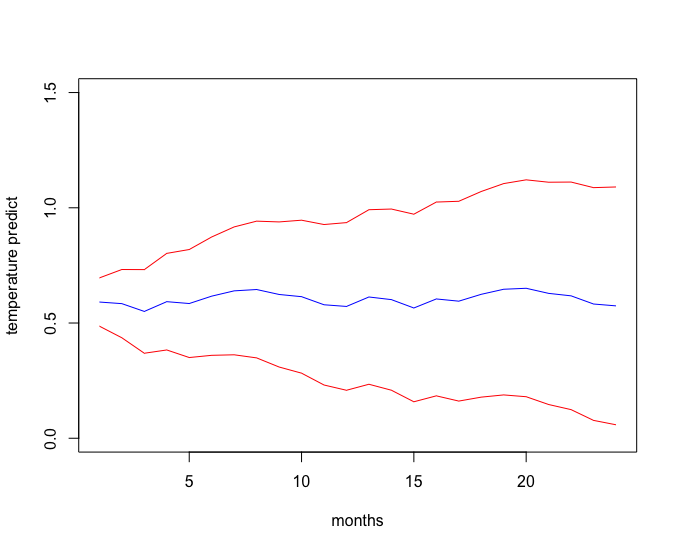
\includegraphics[scale=.40]{predict01.png}
\end{figure}
\end{frame}


\begin{frame}
\frametitle{Conclusion}
sGARCH model can explain the heteroscedastic partially. I've also tried eGARCH model only to find similar results. Next I'll explore long memory model or exclude some extreme values. 
\end{frame}

\begin{frame}

\Huge{\centerline{The End}}

\end{frame}

%----------------------------------------------------------------------------------------

\end{document} 